\documentclass[../../../dissertation.tex]{subfiles}
\begin{document}

Qiskit's \textit{diagonal} function is based on theorem $7$ of \cite{shende06},
where a special case of multiplexors with a single data bit is defined. There,
it is proven that any diagonal gate, $\Delta$, can be expressed as a
multiplexor of diagonal gates, and the decomposition can be seen in figure
\ref{fig:shendeDiagDecomp}. 
%\begin{figure}[!h]
%        \[ \Qcircuit @C=1.5em @R=1.3em {
%                       &   & \multigate{1}{\Delta} &\qw  & &\raisebox{-2.2em}{\equiv} & \\
%                                   &  {/} &\ghost{\Delta} &\qw
%                          }
%          \Qcircuit @C=1.5em @R=1.0em {
%                       &        &\qw     & \gate{R_z} \cwx[1] & \qw \\
%                                   & {/} & \gate{\Delta}    & \controlo  \qw   & \qw
%                          }\]
%        \centering
%        \caption{Decomposition of diagonal operators.}
%        \label{fig:shendeDiagDecomp}
%\end{figure}\par
\begin{figure}[!h]
	\centering
	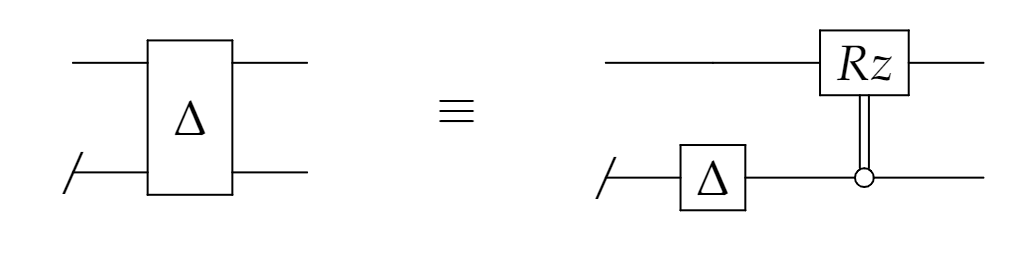
\includegraphics[scale=0.35]{img/QCircuit/diagonal/qcDelta.png}
	\caption{Decomposition of diagonal operators.} 
	\label{fig:shendeDiagDecomp}
\end{figure}\par

For the simple case of a singly-multiplexed $R_z$ gate, theorem 4 of
\cite{shende06} provides a way of demultiplexing this operator, as shown in
figure \ref{fig:shendeSingleRz}.
%\begin{figure}[!h]
%        \[ \Qcircuit @C=1.5em @R=1.3em { 
%                       & \gate{R_z} \cwx[1] &\qw   &\raisebox{-2.2em}{\equiv} & \\
%                       & \controlo  \qw  &\qw
%                          } 
%                \Qcircuit @C=1.5em @R=1.3em { 
%                       & \gate{R_z} &\targ         & \gate{R_z} & \targ    & \qw \\
%                       & \qw        & \ctrl{-1}    &  \qw       & \ctrl{-1} & \qw    
%                          }\]
%        \centering
%        \caption{Decomposition of a singly-multiplexed $R_z$ gate.}
%        \label{fig:shendeSingleRz}
%\end{figure}
\begin{figure}[!h]
	\centering
	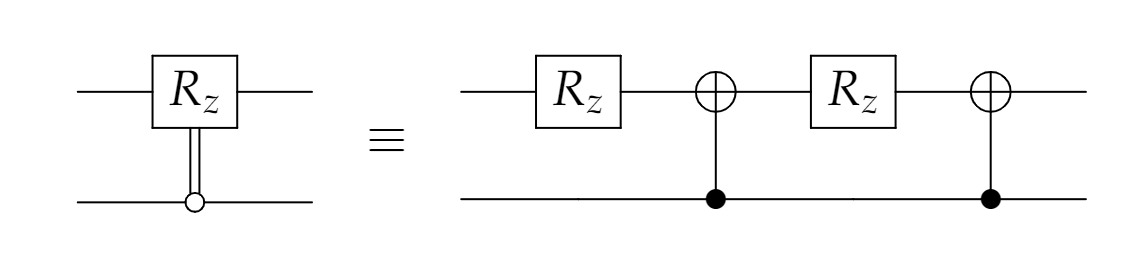
\includegraphics[scale=0.35]{img/QCircuit/diagonal/qcSingDecomp.png}
	\caption{Decomposition of a singly-multiplexed $R_z$ gate.} 
	\label{fig:shendeSingleRz}
\end{figure}
This can then be used to build the general case of the decomposition, as done in theorem
8 of \cite{shende06} and presented in figure \ref{fig:shendeGeneralRz}.
%\begin{figure}[!h]
%        \[ \Qcircuit @C=1.5em @R=1.3em { 
%                      &   & \gate{R_z} \cwx[1]        &\qw   &  &\raisebox{-4.5em}{\equiv} & \\
%                      &{/}& \controlo \cwx[1] \qw     &\qw                              \\
%                      &   & \controlo  \qw            &\qw
%                          } 
%                \Qcircuit @C=1.5em @R=1.3em { 
%                      &   & \gate{R_z} \cwx[1] & \targ        & \gate{R_z}\cwx[1] & \targ     & \qw \\
%                      &{/}& \controlo \qw      & \qw          &  \controlo \qw    & \qw       & \qw\\
%                      &   & \qw                & \ctrl{-2}    &  \qw              & \ctrl{-2} & \qw    
%                          }\]
%        \centering
%        \caption{General decomposition of a multiplexed $R_z$ gate.}
%        \label{fig:shendeGeneralRz}
%\end{figure}
\begin{figure}[!h]
	\centering
	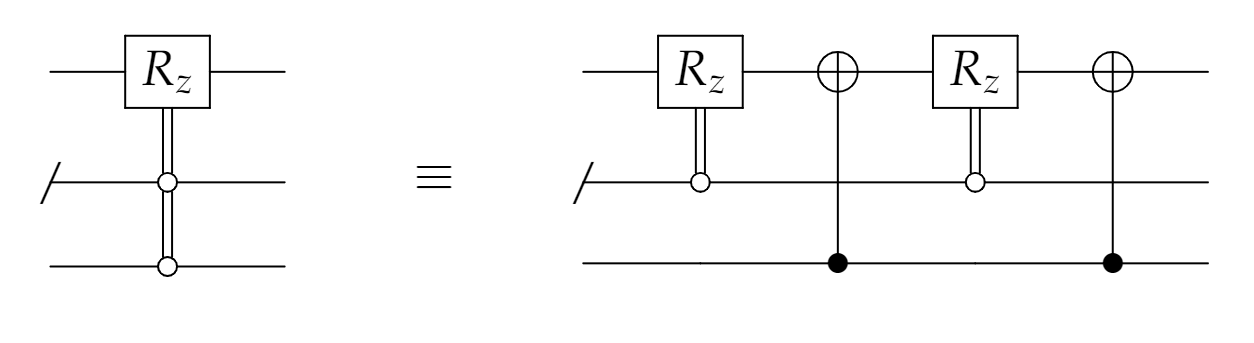
\includegraphics[scale=0.35]{img/QCircuit/diagonal/qcGenDecomp.png}
	\caption{General decomposition of a multiplexed $R_z$ gate.} 
	\label{fig:shendeGeneralRz}
\end{figure}
This method can be used to recursively decompose any multiplexed rotation into basic gates.

\end{document}
